\chapter{HASIL DAN PEMBAHASAN}
\label{chap:hasildanpembahasan}

% Ubah bagian-bagian berikut dengan isi dari pengujian dan analisis


Pada penelitian ini dipaparkan hasil pengujian berupa implementasi Unreal Engine 5 yang dapat menjalankan sistem dari Smart Contract, serta melakukan pengujian terkait
dengan data audio yang diload selama proses sistem berjalan hingga ke tahap pemutaran audio.

\section{Hasil Pembuatan Wallet Account}
Pembuatan wallet account dilakukan dengan Metamask. Pada platform metamask dapat dilakukan pembuatan akun dengan menginstall extension browsernya. Setelah terbuat akunnya maka perlu
digunakan faucet untuk mengisi ETH. ETH yang didapat adalah sejumlah 13 GoerliETH. ETH ini sudah lebih dari cukup untuk digunakan. Kemudian dibuat juga akun kedua dan diisikan dengan GoerliETH.
Akun kedua juga dapat digunakan untuk pengujian.

\section{Hasil Pembuatan Smart Contract}
Smart Contract yang dibuat dapat digunakan untuk mint NFT. Deployment dilakukan dengan Environment Injected Provider Metamask.
Metamask yang digunakan adalah akun yang sudah dibuat sebelumnya. Contract yang dibuat dideploy sudah digunakan untuk mint NFT.

\section{Hasil Pembuatan Metadata dengan IPFS}
Metadata yang dibuat di IPFS sudah dapat diakses melalui gatewaynya. Contohnya untuk nft-1.json adalah sebagai berikut.

\begin{figure}[H]
  \centering

  % Ubah dengan nama file gambar dan ukuran yang akan digunakan
  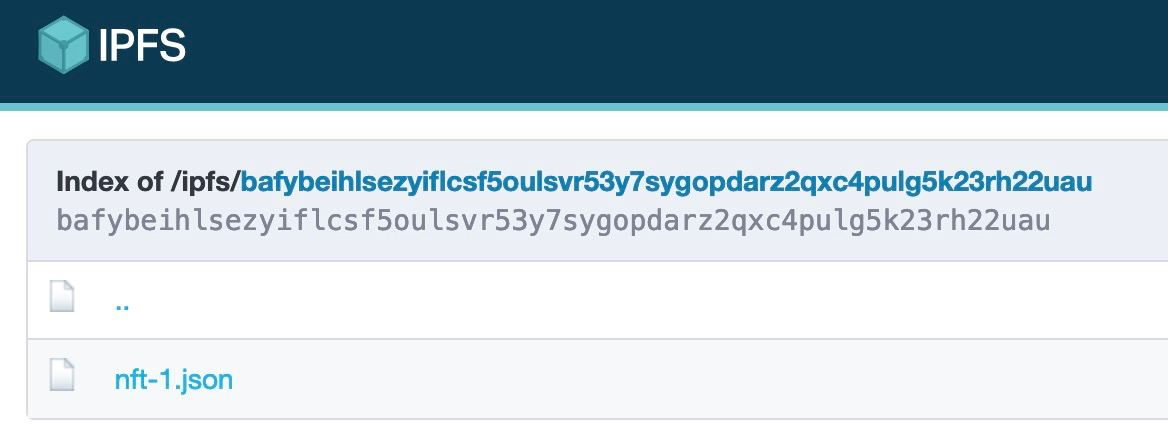
\includegraphics[scale=0.3]{gambar/nftjsonuploaded.jpg}

  % Ubah dengan keterangan gambar yang diinginkan
  \caption{Tampilan IPFS nft-1.json yang sudah diupload}
  \label{fig:ipfsjsonuploaded}
\end{figure}

\section{Hasil Mint NFT}
Hasil dari mint nft sudah dapat digunakan untuk integrasi Unreal Engine 5. ABI dapat dilihat pada compiler Remix IDE.
\begin{figure}[H]
  \centering

  % Ubah dengan nama file gambar dan ukuran yang akan digunakan
  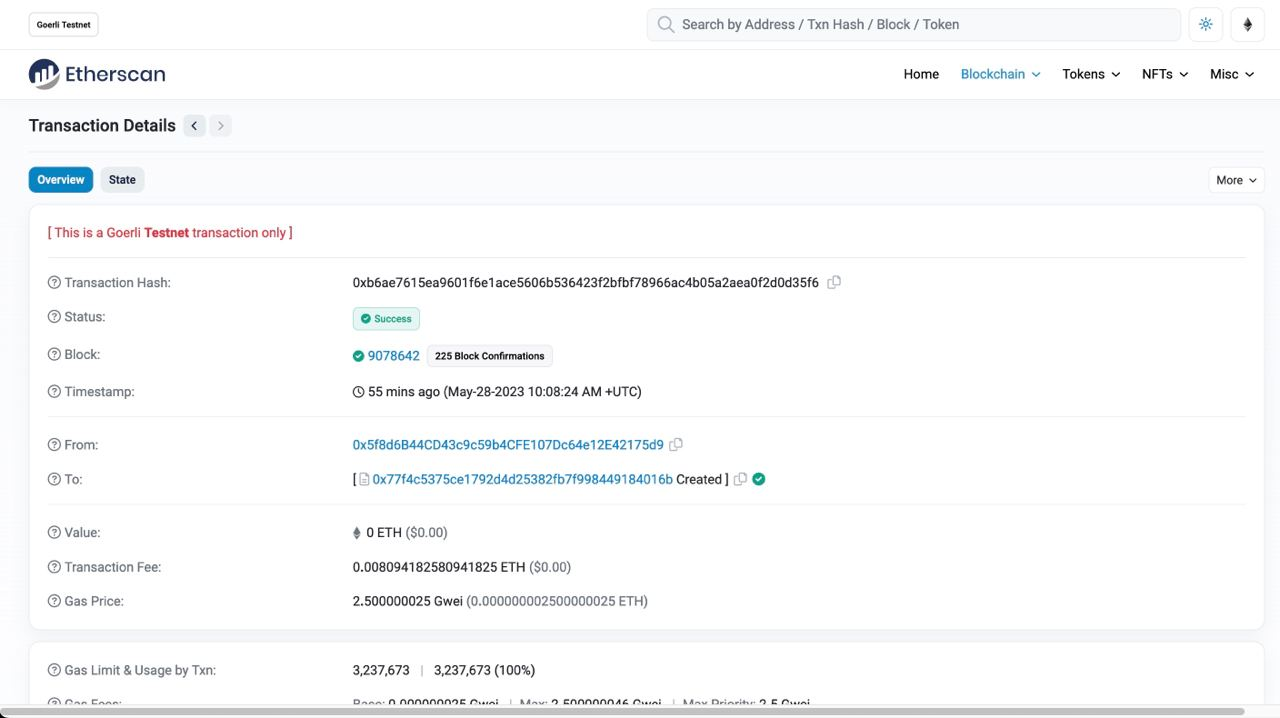
\includegraphics[scale=0.3]{gambar/etherscan-deploy.jpg}

  % Ubah dengan keterangan gambar yang diinginkan
  \caption{Etherscan dari hasil transaction mint NFT}
  \label{fig:etherscandeploy}
\end{figure}

\section{Hasil Pembuatan Project Pada Unreal Engine 5}
Project unreal engine 5 yang sudah dibuat dapat memberikan environment visual yang dapat melakukan visualisasi audio maupun game.

\begin{figure}[H]
  \centering

  % Ubah dengan nama file gambar dan ukuran yang akan digunakan
  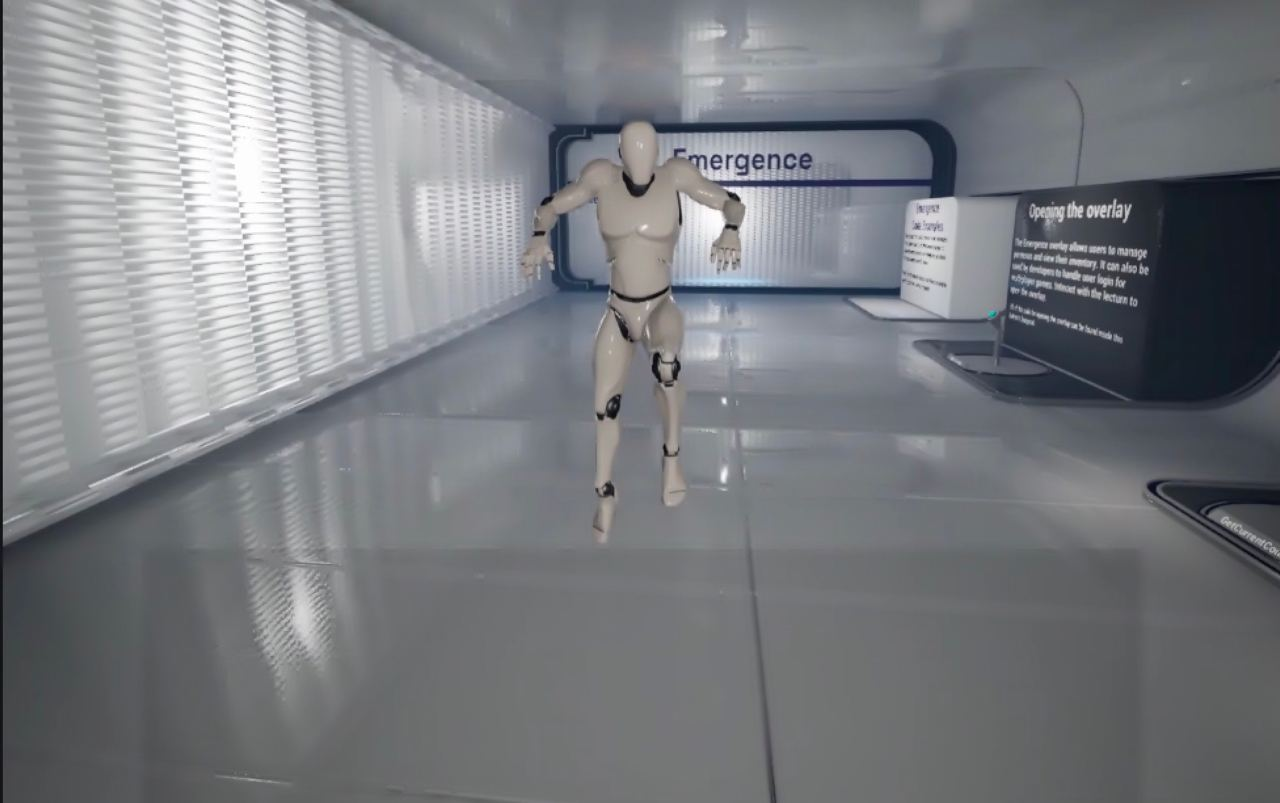
\includegraphics[scale=0.3]{gambar/ue5project.jpg}

  % Ubah dengan keterangan gambar yang diinginkan
  \caption{Tampilan project unreal engine 5}
  \label{fig:ue5project}
\end{figure}

\section{Hasil Integrasi Kontrak dengan Unreal Engine 5}

Setelah diintegrasikan dengan blueprint maka di lingkungan virtual unreal engine 5 sudah dapat memutar audio yang didapatkan dari NFT.
Blueprint yang digunakan adalah sebagai berikut.

\begin{figure}[H]
  \centering

  % Ubah dengan nama file gambar dan ukuran yang akan digunakan
  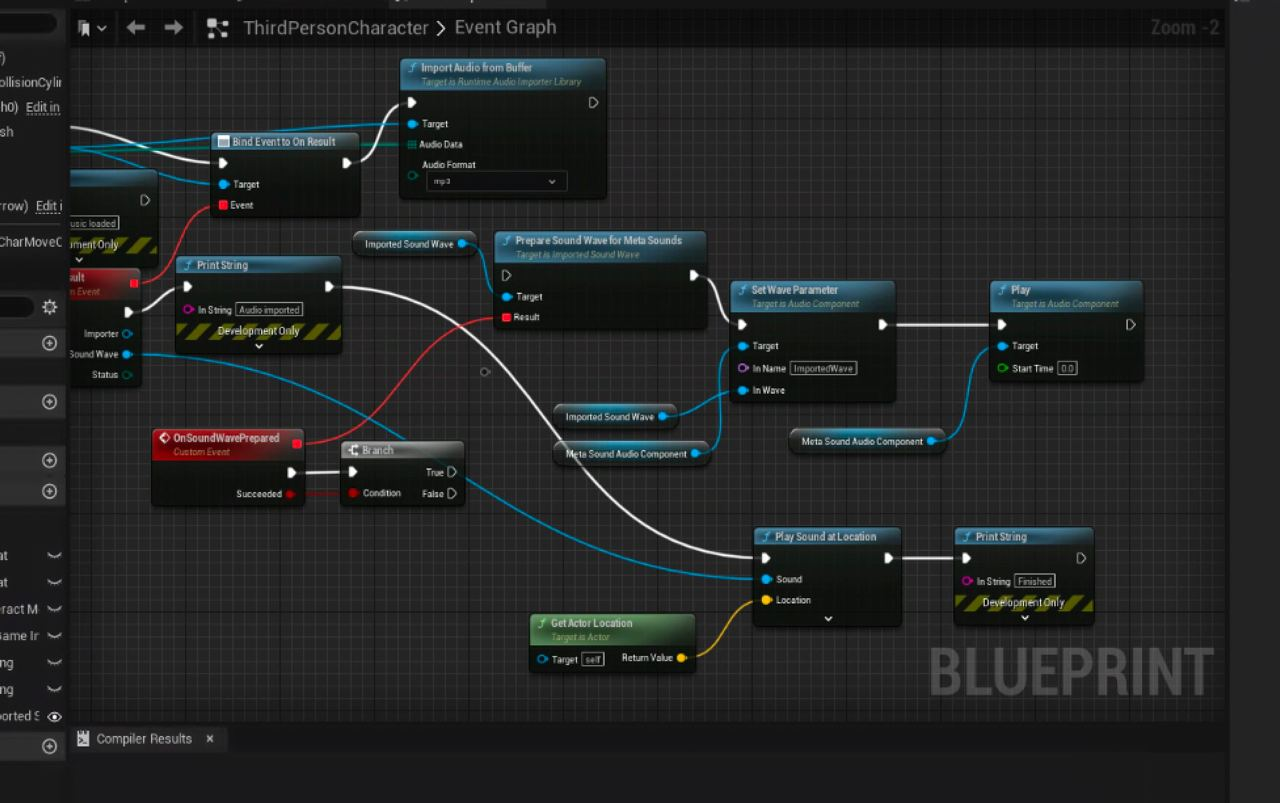
\includegraphics[scale=0.3]{gambar/blueprintfinal.jpg}

  % Ubah dengan keterangan gambar yang diinginkan
  \caption{Tampilan blueprint final}
  \label{fig:blueprintfinal}
\end{figure}
